\documentclass[11pt,a4paper]{article}
\usepackage[T1]{fontenc}
\usepackage[utf8]{inputenc}
\usepackage{lmodern}
\usepackage[margin=22mm,headheight=16pt]{geometry}
\usepackage{amsmath,amssymb,graphicx,array,longtable,booktabs}
\usepackage{microtype,xcolor,hyperref,xurl,fancyhdr}
\definecolor{Navy}{HTML}{17324D}
\definecolor{Teal}{HTML}{087F8C}
\definecolor{Gold}{HTML}{B88128}
\hypersetup{colorlinks=true,linkcolor=Navy,urlcolor=Teal,bookmarksnumbered=true,hypertexnames=false}
\setlength{\parindent}{0pt}
\setlength{\parskip}{6pt}
\setlength{\emergencystretch}{4em}
\setcounter{tocdepth}{1}
\pagestyle{fancy}\fancyhf{}
\fancyfoot[R]{\small\thepage}
\fancyfoot[L]{\small\sffamily Sharif University of Technology}
\renewcommand{\headrulewidth}{0.3pt}
\makeatletter
\renewcommand\section{\@startsection{section}{1}{\z@}{-3.2ex plus -1ex minus -.2ex}{1.6ex plus .2ex}{\normalfont\Large\sffamily\bfseries\color{Navy}}}
\renewcommand\subsection{\@startsection{subsection}{2}{\z@}{-2.5ex plus -1ex minus -.2ex}{1.2ex plus .2ex}{\normalfont\large\sffamily\bfseries\color{Teal}}}
\makeatother
\fancyhead[L]{\small\sffamily\color{Navy}Reza Sanaee Nezhad}\fancyhead[R]{\small\sffamily\color{Teal}Technical Report}\begin{document}
\begin{titlepage}\centering\vspace*{7mm}

\includegraphics[width=31mm]{assets/sharif_emblem_en.png}\par\vspace{5mm}
{\Large\sffamily\bfseries\color{Navy}SHARIF UNIVERSITY OF TECHNOLOGY\par}
\vspace{2mm}{\sffamily Department of Electrical Engineering\par}
\vspace{17mm}{\color{Teal}\rule{\linewidth}{1.4pt}}\par\vspace{6mm}
{\large\sffamily\color{Teal}TECHNICAL REPORT\par}
\vspace{8mm}{\huge\sffamily\bfseries\color{Navy}Folded-Cascode Amplifier Redesign with Class-B Output\par}
\vspace{9mm}{\color{Gold}\rule{45mm}{1pt}}\par\vfill
\begin{minipage}{.88\linewidth}{\sffamily\color{Teal}AUTHOR}\par{\Large\sffamily Reza Sanaee Nezhad}\par Student ID: 401101502\par\vspace{7mm}
{\sffamily\color{Teal}INSTRUCTOR / INSTRUCTORS}\par
Dr Mohammad Fakharzadeh; Dr Reza Sarvari; Dr Ali Maddi\par\vspace{7mm}
{\sffamily\color{Teal}ACADEMIC CONTEXT}\par
Electronics II\par\end{minipage}\vfill
\end{titlepage}
\tableofcontents\clearpage
\section{Initial topology and bias analysis}

The initial input is a cascoded differential stage formed by Q1-Q4. Q7-Q8 form a complementary class-B push-pull output. Q6 affects the output-stage bias and DC level;\allowbreak{} IB also affects whether Q5 conducts. The recorded KCL expression at B gives -IB6-IC5+\allowbreak{}IB-I=\allowbreak{}0, with approximate base current 1.33 uA and resistor current 67 uA. Positive IC5 therefore requires IB greater than approximately 68.33 uA. The report's prose proposes 2 mA but its following operating-point calculation uses 0.2 mA;\allowbreak{} these are different assumptions, and the reproduced table belongs to the latter. With the recorded approximation VBE=\allowbreak{}0.67 V and IB=\allowbreak{}0.2 mA, the report obtains IC5 approximately 0.132 mA and IC6=\allowbreak{}0.2 mA. Its branch equations give IC2=\allowbreak{}IC4=\allowbreak{}0.8 mA and IC1=\allowbreak{}IC3=\allowbreak{}1.2 mA. At zero input it assumes the ideal class-B output devices carry zero current.


\begingroup\small\setlength{\tabcolsep}{3pt}\renewcommand{\arraystretch}{1.2}
\begin{longtable}{@{}p{0.3100\linewidth}p{0.3100\linewidth}p{0.3100\linewidth}@{}}
\toprule
\textbf{Device} & \textbf{IC (mA), submitted approximation} & \textbf{Signed VCE (V), submitted approximation} \\ \midrule
\endfirsthead
\textbf{Device} & \textbf{IC (mA), submitted approximation} & \textbf{Signed VCE (V), submitted approximation} \\ \midrule \endhead
Q1 & 1.2 & 4 \\
Q2 & 0.8 & 4 \\
Q3 & 1.2 & 6.67 \\
Q4 & 0.8 & 0.69 \\
Q5 & 0.132 & 5.36 \\
Q6 & 0.2 & -9.33 \\
Q7 & 0 & 10 \\
Q8 & 0 & -10 \\
\bottomrule\end{longtable}\endgroup

The table preserves the submitted signed-voltage convention and approximate transistor model. Negative PNP VCE does not itself mean a negative headroom magnitude;\allowbreak{} device polarity and terminal convention must be considered. Actual operating points should be taken from a consistent SPICE .op run before confirming every region-of-operation assumption.

\[ P_{\rm load}=\frac{V_{\rm peak}^2}{2R}=\frac{8.2^2}{200}=0.3362\ \mathrm{W}. \]
\section{Dead zone, feedback, and initial swing}

In a class-B pair, a small input around the switching region may leave neither output transistor strongly conducting, causing crossover distortion. Negative feedback can reduce the output error while the loop retains sufficient gain and bandwidth, but cannot guarantee perfectly linear operation or remove all distortion. The recorded node-X and output plots with approximately 1-mV excitation illustrate the feedback response and an approximately twofold output. The report estimates a positive output limit of 0.2 mA times beta=\allowbreak{}200 times 100 ohms, or 4 V, and a negative limit near -0.49 V from its headroom equations. Those asymmetric limits should not be summarized as a symmetric peak-to-peak swing without qualification. A zero-centered sine would be limited by the smaller magnitude, giving approximately 0.98 V peak-to-peak under that assumption. The submitted input common-mode expressions produce an upper limit of 10.27 V and lower limit -9.8 V. A limit above the +\allowbreak{}10-V rail is not established by that simplified equation and is flagged as inconsistent with an unverified transistor-headroom analysis. The source screenshots and equations are preserved rather than replaced with an invented simulated ICMR.

\begin{figure}[!htbp]\centering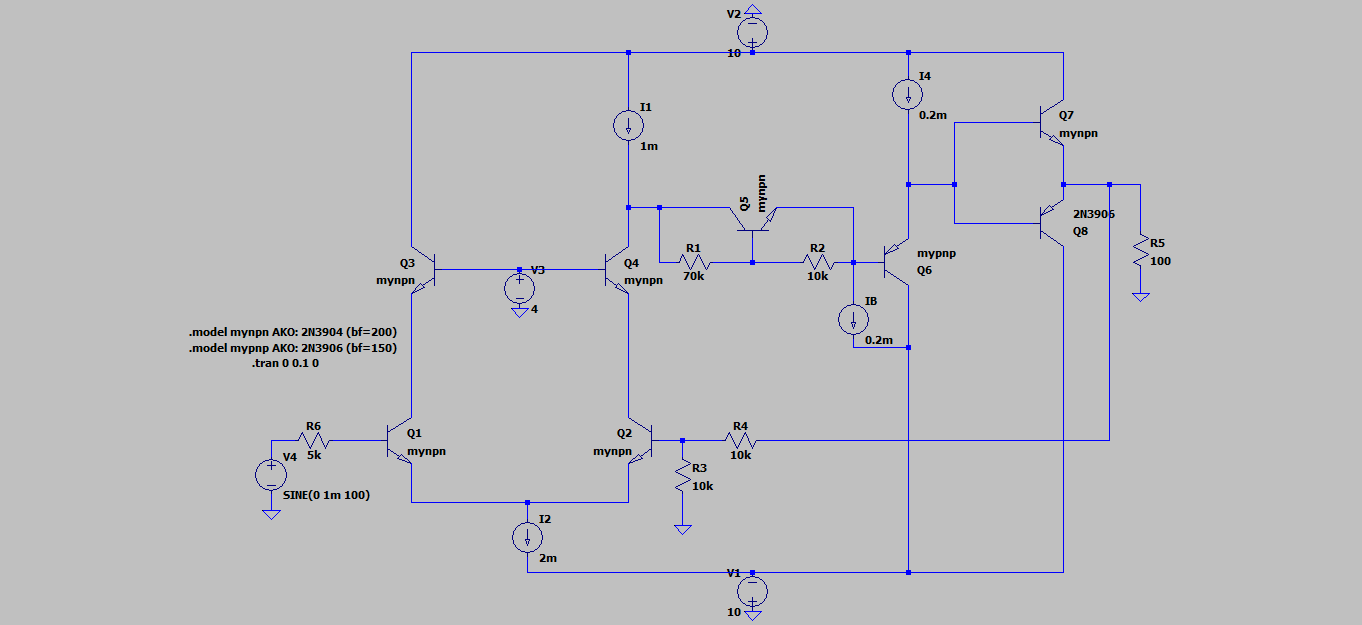
\includegraphics[width=\linewidth,height=.72\textheight,keepaspectratio]{assets/029_p003_01.png}\caption{Diagram or recorded result: Dead zone, feedback, and initial swing.}\label{fig:029_p003_010}\end{figure}
\clearpage
\section{Preliminary operating-point change and THD}

Increasing the nearby bias current to 0.5 mA and reducing the input-stage bias voltage to 2 V increases the reported waveform span to approximately 10 V peak-to-peak. THD is the square root of the summed squared RMS higher-harmonic amplitudes divided by the fundamental RMS amplitude, multiplied by 100 percent when expressed as a percentage. The initial FFT evaluation reports approximately 28 percent. A meaningful measurement should specify fundamental frequency, transient settling, FFT interval/\allowbreak{}window, amplitude, and number of harmonics.

\begin{figure}[!htbp]\centering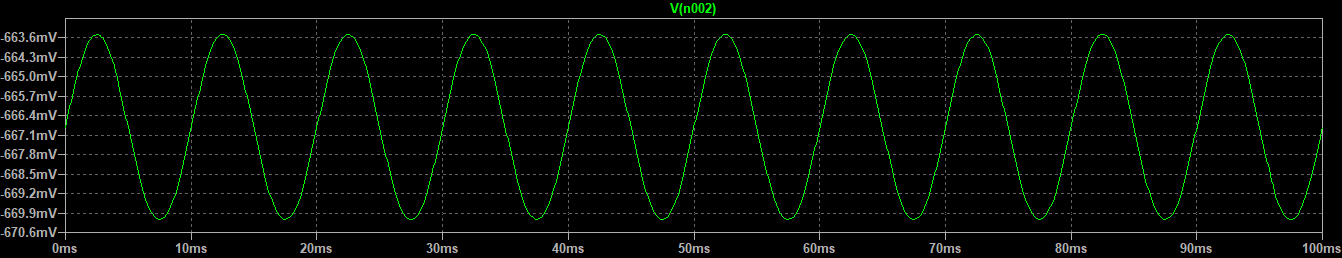
\includegraphics[width=\linewidth,height=.72\textheight,keepaspectratio]{assets/029_p004_01.png}\caption{Diagram or recorded result: Preliminary operating-point change and THD.}\label{fig:029_p004_010}\end{figure}
\begin{figure}[!htbp]\centering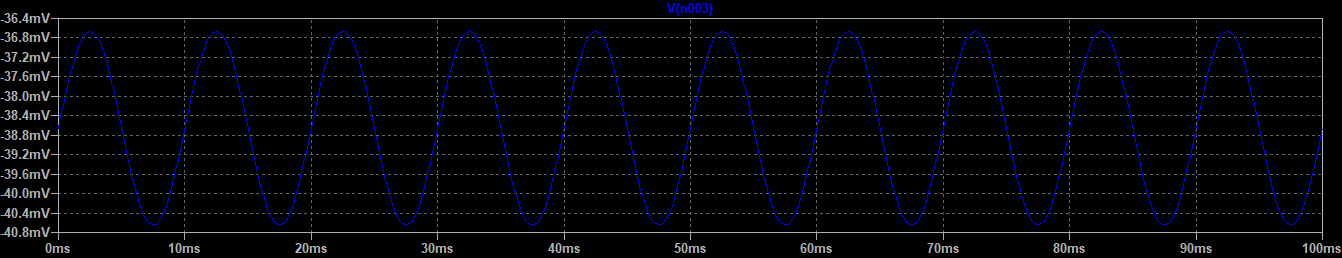
\includegraphics[width=\linewidth,height=.72\textheight,keepaspectratio]{assets/029_p004_02.png}\caption{Diagram or recorded result: Preliminary operating-point change and THD.}\label{fig:029_p004_020}\end{figure}
\begin{figure}[!htbp]\centering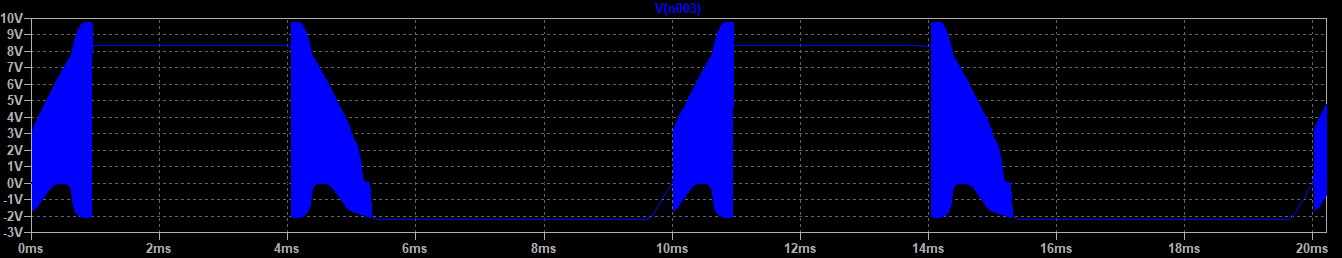
\includegraphics[width=\linewidth,height=.72\textheight,keepaspectratio]{assets/029_p004_03.png}\caption{Diagram or recorded result: Preliminary operating-point change and THD.}\label{fig:029_p004_030}\end{figure}
\clearpage
\section{Folded-cascode design and current mirrors}

The recorded redesign replaces the input stage with a folded cascode and replaces four ideal current sources with mirror-based circuits. Folded cascodes can provide high gain and useful voltage headroom, but noise, stability, bandwidth, and supply sensitivity depend on the actual implementation rather than being universally improved by the topology name. The report begins with an approximate resistance/\allowbreak{}current relation R times I approximately 20 V. A more precise mirror-reference estimate accounts for junction drops, current gain, and output compliance. It uses 9.65 kohm to obtain an approximately 2-mA reference, adjusts input/\allowbreak{}folded branches toward a combined 8 mA, raises a cascode-related base level toward 9 V to increase headroom, and discusses a nominal 20-mA mirror with R=\allowbreak{}1 kohm. It also lowers interstage resistances to reduce voltage drop and changes one output transistor's IS parameter as permitted. These are the submitted design decisions;\allowbreak{} their exact implementation remains visible in the full schematic and supplied .asc files.

\begin{figure}[!htbp]\centering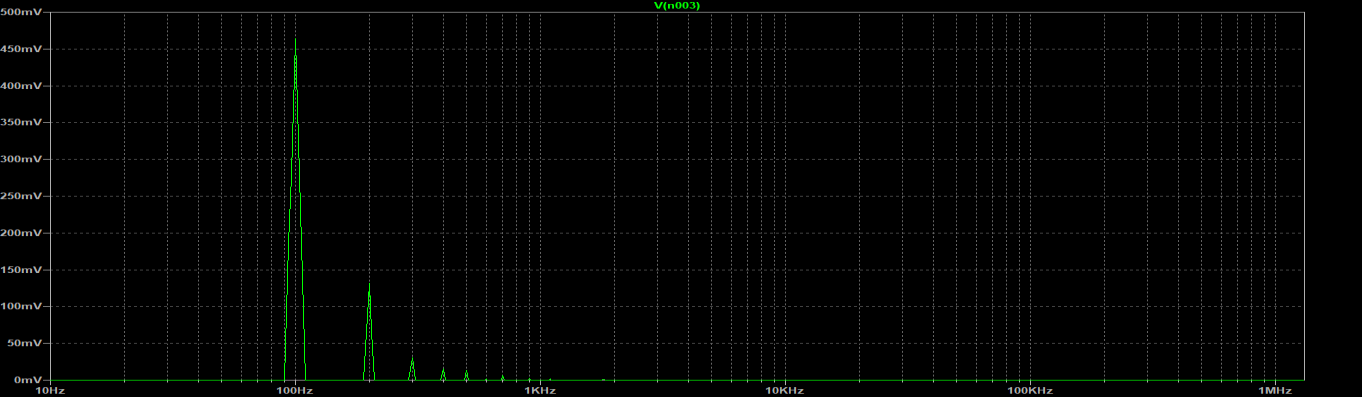
\includegraphics[width=\linewidth,height=.72\textheight,keepaspectratio]{assets/029_p005_01.png}\caption{Diagram or recorded result: Folded-cascode design and current mirrors.}\label{fig:029_p005_010}\end{figure}
\clearpage
\section{Redesigned measurements and compliance}

\begingroup\small\setlength{\tabcolsep}{3pt}\renewcommand{\arraystretch}{1.2}
\begin{longtable}{@{}p{0.2263\linewidth}p{0.2263\linewidth}p{0.2263\linewidth}p{0.2263\linewidth}@{}}
\toprule
\textbf{Quantity} & \textbf{Reported result} & \textbf{Required value} & \textbf{Assessment} \\ \midrule
\endfirsthead
\textbf{Quantity} & \textbf{Reported result} & \textbf{Required value} & \textbf{Assessment} \\ \midrule \endhead
Closed-loop gain & Approximately 2 & 2 & Demonstrated in the supplied waveform \\
Output swing & 17.072 V peak-to-peak & Greater than 16.6 V peak-to-peak & Recorded value exceeds target \\
Quiescent power & 61 mW & At most 50 mW & Fails by 11 mW, or 22 percent \\
THD at 16.4 V peak-to-peak & Approximately 1 percent & Below 0.05 percent & About twenty times the limit \\
\bottomrule\end{longtable}\endgroup

Reduced distortion from the initial 28-percent result is still a design improvement, but not specification compliance. At +\allowbreak{}/\allowbreak{}-8.2 V across 100 ohms, sinusoidal load power is 8.2 squared divided by 200, or 0.3362 W. This delivered signal power is distinct from the no-input quiescent power.

\begin{figure}[!htbp]\centering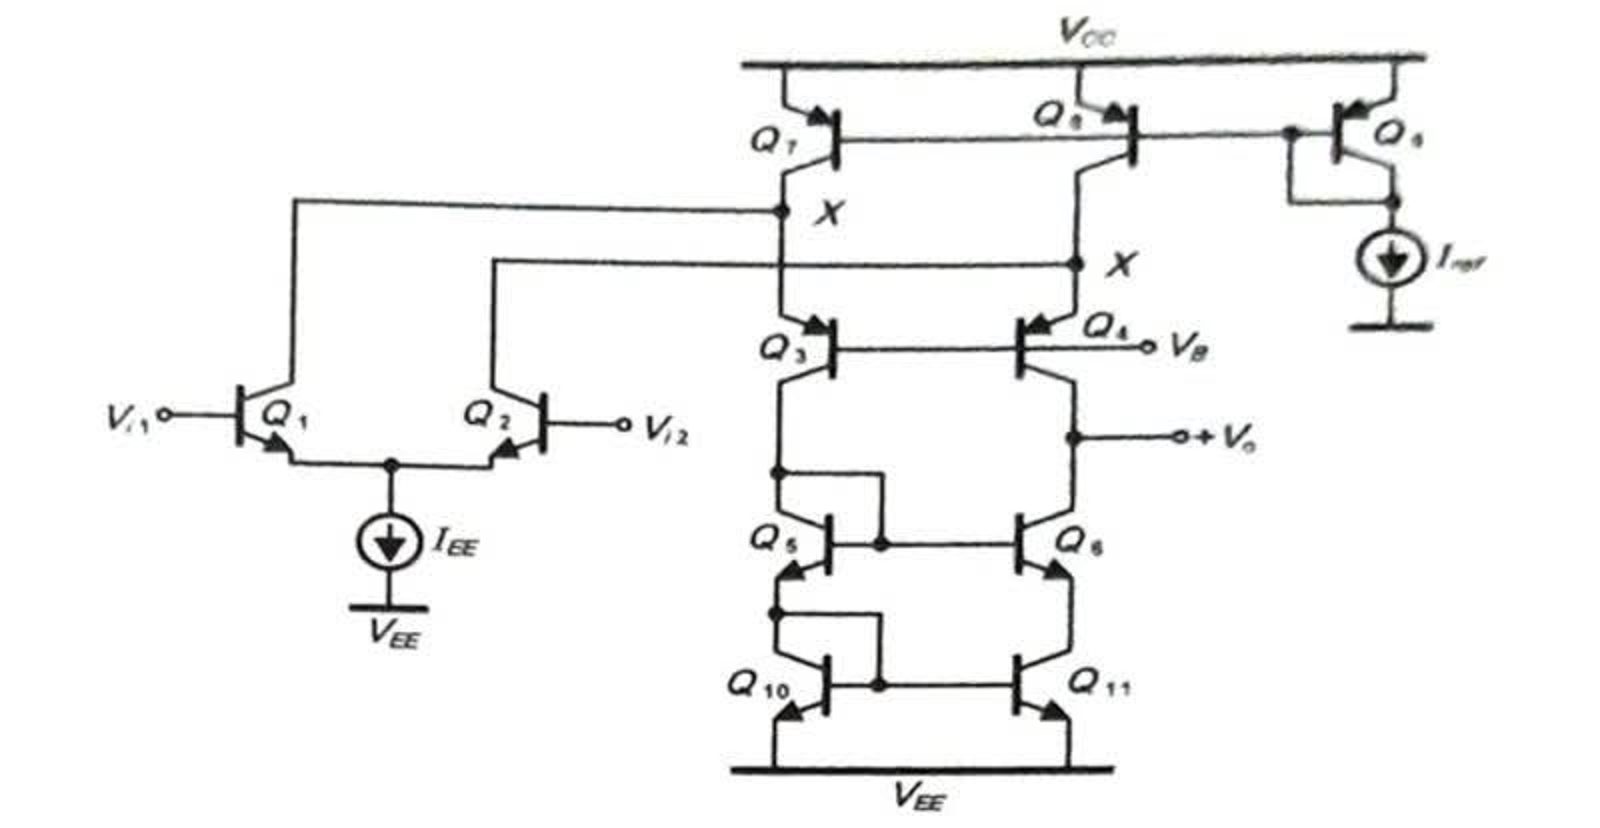
\includegraphics[width=\linewidth,height=.72\textheight,keepaspectratio]{assets/029_p006_01.png}\caption{Diagram or recorded result: Redesigned measurements and compliance.}\label{fig:029_p006_010}\end{figure}
\begin{figure}[!htbp]\centering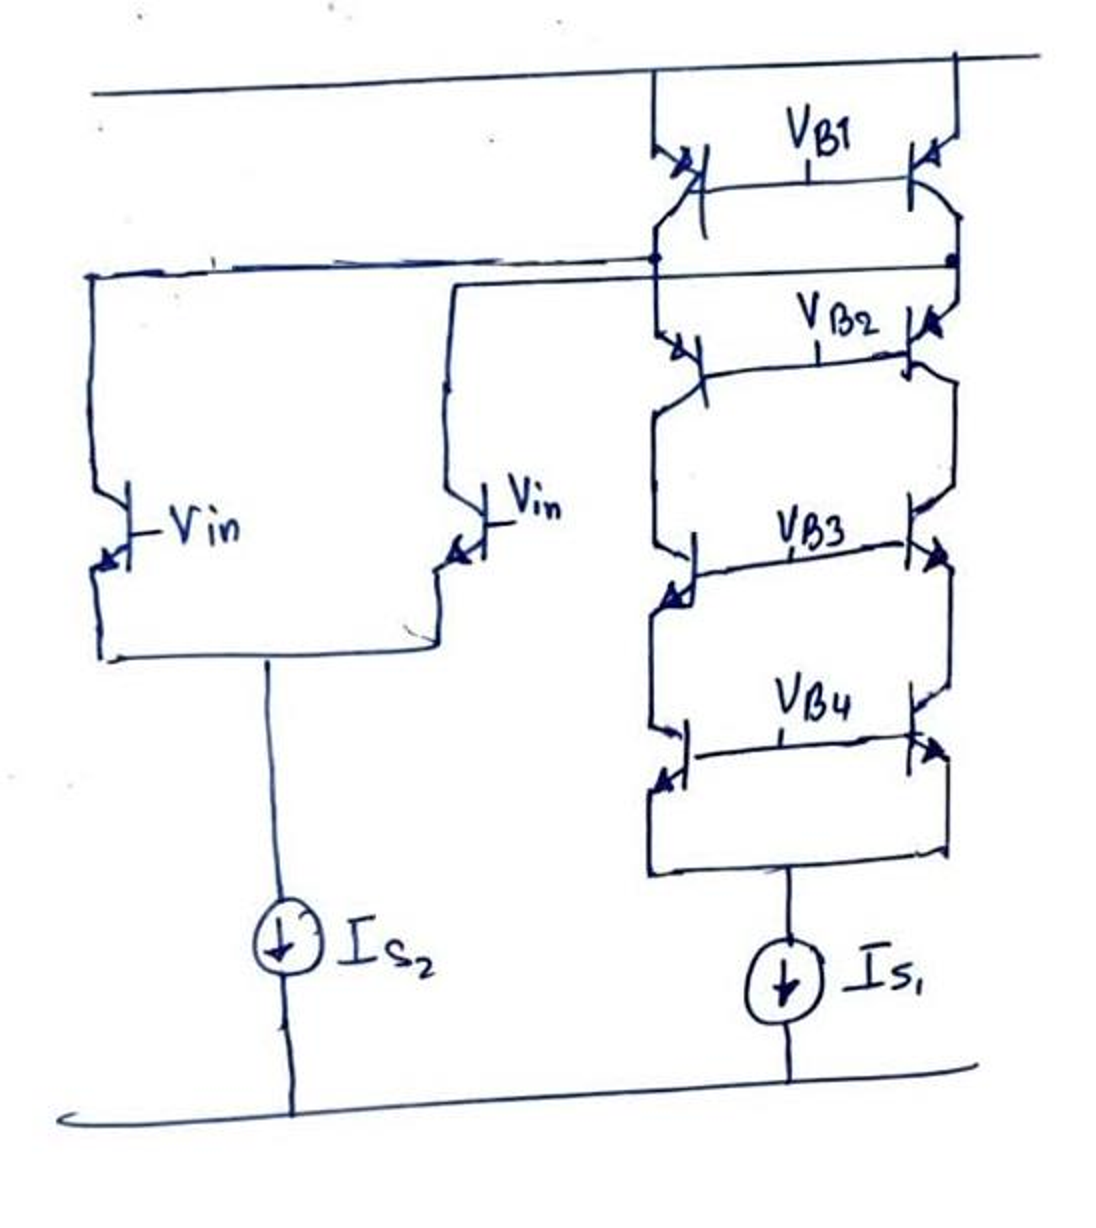
\includegraphics[width=\linewidth,height=.72\textheight,keepaspectratio]{assets/029_p006_02.png}\caption{Diagram or recorded result: Redesigned measurements and compliance.}\label{fig:029_p006_020}\end{figure}
\begin{figure}[!htbp]\centering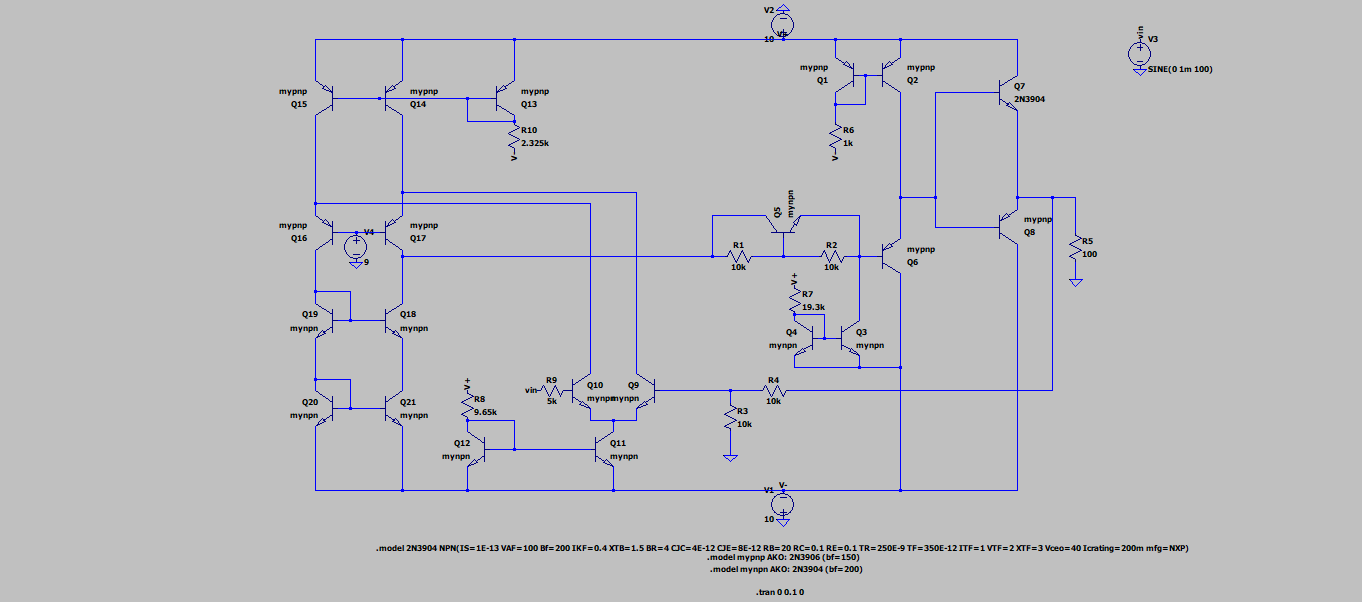
\includegraphics[width=\linewidth,height=.72\textheight,keepaspectratio]{assets/029_p007_01.png}\caption{Diagram or recorded result: Redesigned measurements and compliance.}\label{fig:029_p007_010}\end{figure}
\begin{figure}[!htbp]\centering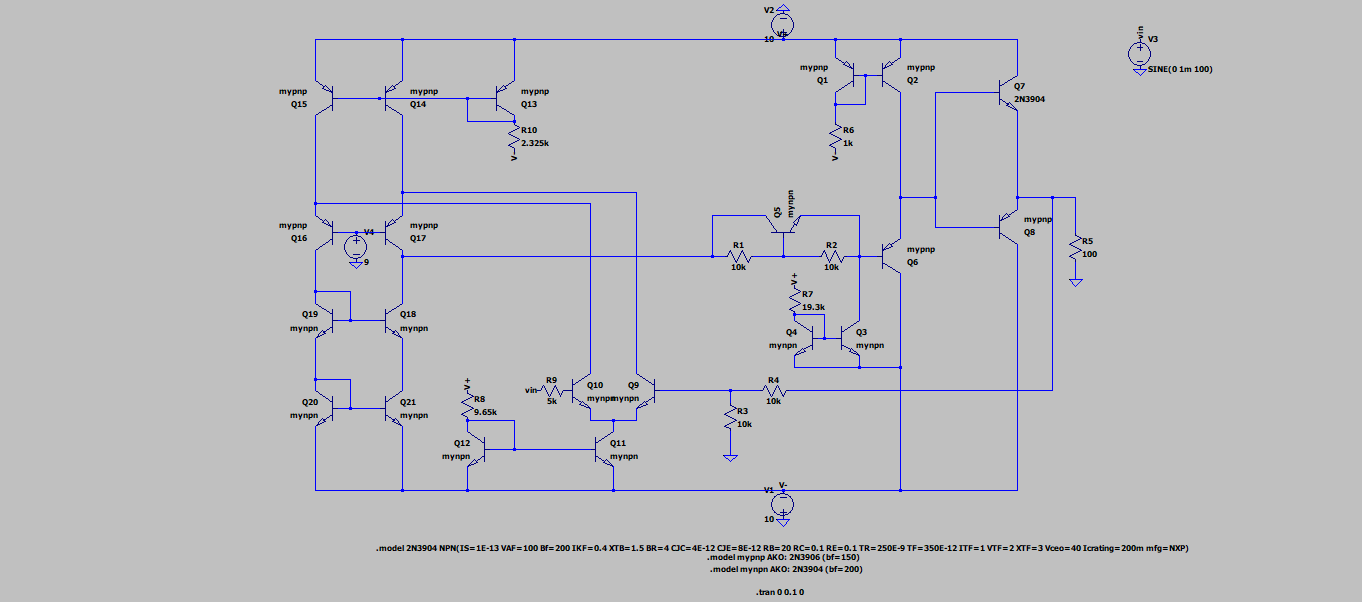
\includegraphics[width=\linewidth,height=.72\textheight,keepaspectratio]{assets/029_p008_01.png}\caption{Diagram or recorded result: Redesigned measurements and compliance.}\label{fig:029_p008_010}\end{figure}
\begin{figure}[!htbp]\centering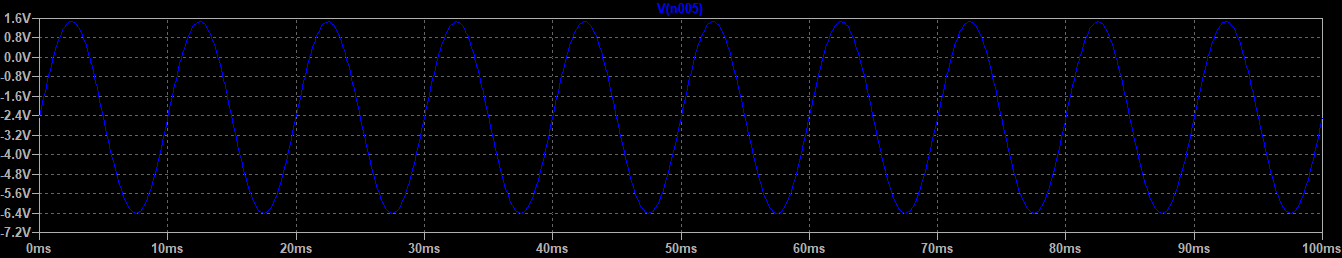
\includegraphics[width=\linewidth,height=.72\textheight,keepaspectratio]{assets/029_p008_02.png}\caption{Diagram or recorded result: Redesigned measurements and compliance.}\label{fig:029_p008_020}\end{figure}
\begin{figure}[!htbp]\centering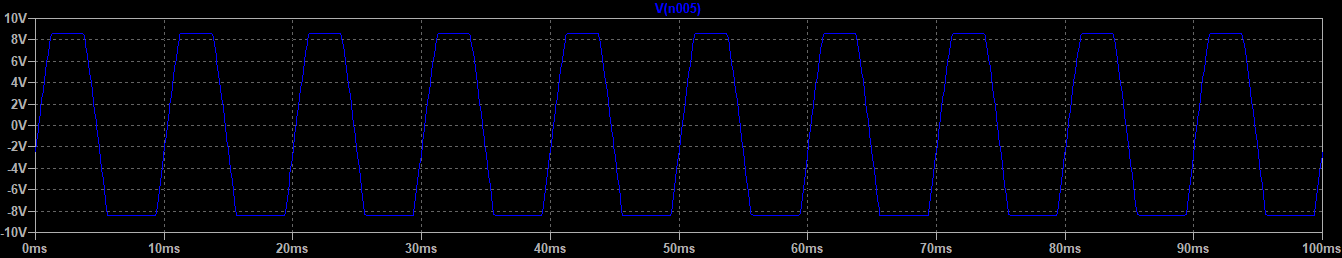
\includegraphics[width=\linewidth,height=.72\textheight,keepaspectratio]{assets/029_p008_03.png}\caption{Diagram or recorded result: Redesigned measurements and compliance.}\label{fig:029_p008_030}\end{figure}
\clearpage
\section{Feedback-resistor experiment and remaining questions}

For the final resistor-change experiment, the input is reduced to approximately 2 V because larger inputs produce clipping or nonlinear behavior. The distortion discussion considers the feedback network and differential-input resistance. A controlled parameter comparison would be needed to attribute the measured THD to a single cause. That is not a complete circuit derivation:\allowbreak{} input currents, feedback loading, loop gain, bias shifts, slew/\allowbreak{}range limits, and resistor noise can contribute and must be tested in the actual model. The two LTspice models are organized as simulation source, and no replacement simulation has been claimed.

\begin{figure}[!htbp]\centering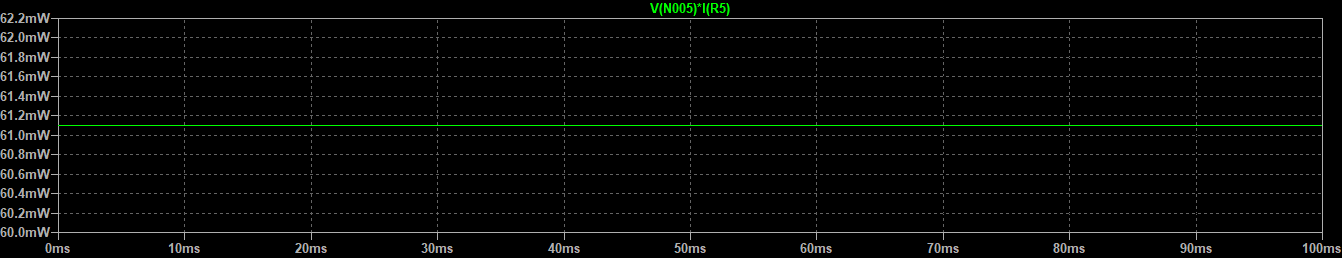
\includegraphics[width=\linewidth,height=.72\textheight,keepaspectratio]{assets/029_p009_01.png}\caption{Diagram or recorded result: Feedback-resistor experiment and remaining questions.}\label{fig:029_p009_010}\end{figure}
\begin{figure}[!htbp]\centering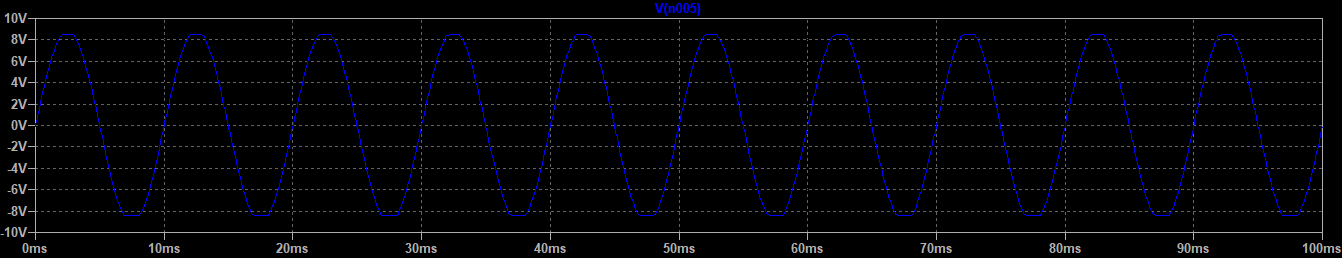
\includegraphics[width=\linewidth,height=.72\textheight,keepaspectratio]{assets/029_p009_02.png}\caption{Diagram or recorded result: Feedback-resistor experiment and remaining questions.}\label{fig:029_p009_020}\end{figure}
\begin{figure}[!htbp]\centering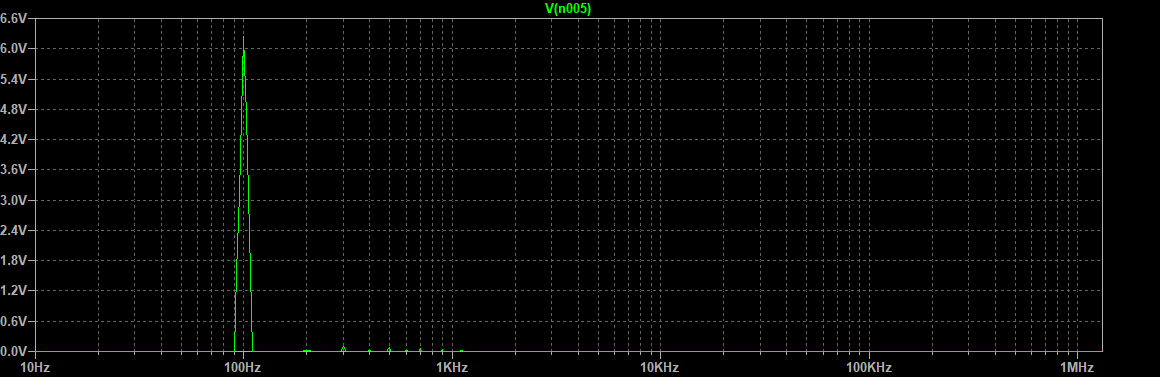
\includegraphics[width=\linewidth,height=.72\textheight,keepaspectratio]{assets/029_p009_03.png}\caption{Diagram or recorded result: Feedback-resistor experiment and remaining questions.}\label{fig:029_p009_030}\end{figure}
\begin{figure}[!htbp]\centering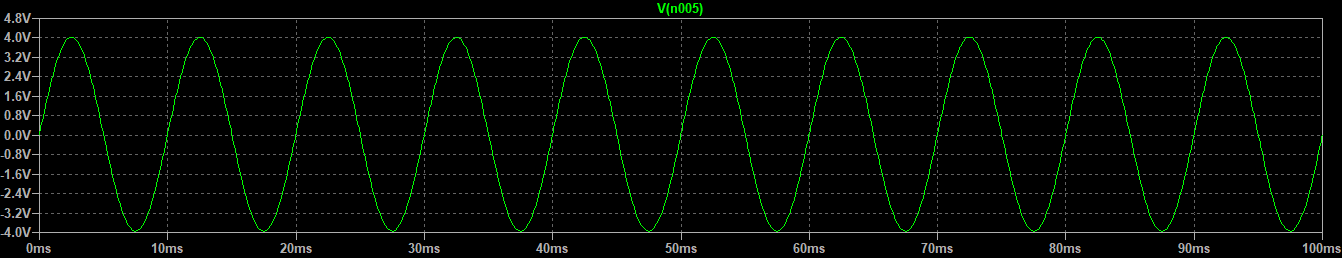
\includegraphics[width=\linewidth,height=.72\textheight,keepaspectratio]{assets/029_p010_01.png}\caption{Diagram or recorded result: Feedback-resistor experiment and remaining questions.}\label{fig:029_p010_010}\end{figure}
\clearpage
\end{document}